\documentclass[a4paper, svgnames]{article}

\usepackage[a4paper, margin=1in]{geometry}
\usepackage[english]{babel}
\usepackage[utf8x]{inputenc}
\usepackage{amsmath}
\usepackage{graphicx}
\usepackage[colorinlistoftodos]{todonotes}
\usepackage{sectsty}
\usepackage{float}
\usepackage{natbib}
\usepackage{url}
\usepackage[colorlinks]{hyperref}
\usepackage{xcolor}
\usepackage{amsmath}
\usepackage{longtable}
\setlength\LTcapwidth{\textwidth}
\usepackage{pdflscape}
\usepackage{booktabs}
\usepackage{afterpage}
\usepackage[bottom]{footmisc}
\usepackage{tikz}

\usepackage{enumitem}
\usepackage{bibspacing}
\setlength{\bibitemsep}{0\baselineskip plus .05\baselineskip minus .05\baselineskip}
\usepackage{rotating, float, placeins}
\usepackage{threeparttable}
\widowpenalty10000
\clubpenalty10000

% Node styles
\tikzstyle{basic box}=[fill=none, draw=black, shape=rectangle]

% Edge styles
\tikzstyle{basic arrow}=[fill=black, ->]

\hypersetup{
    colorlinks,
    citecolor=Blue,
    linkcolor=Blue}

\linespread{1.25}
\sectionfont{\large}
\setlength{\parskip}{1mm}

\newcommand{\citeposs}[1]{\citeauthor{#1}'s \citeyearpar{#1}}
\newcommand{\citepos}[1]{\citeauthor{#1}' \citeyearpar{#1}}

\title{\vspace{-40pt}\textbf{The consequences of affective polarization\\ \Large Is accountability still working?}}
\author{Rodrigo Fernández Caba}
\date{\vspace{-5pt} November, 2021}

\begin{document}
\maketitle

\begin{abstract}
Affective polarization has become the political phenomenon of the moment. Although specially American scholars have studied thoroughly its causes, less effort has been devoted to explain its consequences. In order to do so, I propose a causal mechanism through which affective polarization impacts political attitudes. By a process of motivated reasoning, more polarized people are expected to a) assess incumbent's performances worse, b) form political preferences (i.e. public policy choice) in a perhaps pernicious way for them, and c) be less supportive in general for incumbent's measures (specially during times of crisis). In this paper, I propose to test empirically the first of these effects, namely, the impact of affective polarization on economic voting. My hypothesis is that those who are more polarized will be less rational or, in other words, they will be less able to reward or punish the incumbent according to economic events. Hence, this paper tries to make a contribution to our knowledge of affective polarization and speaks to the general problem of accountability in our contemporary polarized societies.
\end{abstract}


\section{Introduction}

Some scholars have recently pointed out that American people are far more polarized than 40 years ago \citep{Lelkes2018}. Since the seminal piece of work by \cite{Iyengar2012} we know that political polarization is not only related to ideology but also to affects. Inter-party animosity has been increasing at least since the 1980s in American politics. Nonetheless, some others have shown that United States is by no means the most polarized nation around the world. From a comparative perspective, (\citeauthor{Gidron2018} \citeyear{Gidron2018} and \citeyear{Gidron2019}, and \cite{WESTWOOD2018}) (see Figure \ref{fig:af-pol-comp}) have pointed out that whereas Americans display just average levels of affective polarization, in Europe, we find much higher levels, for instance, in countries like Spain, Greece or even France. The ugly discourse surrounding recent elections in the US, the Brexit campaign, or the Community of Madrid electoral campaign in a frame with only two apparent options `Communism or Freedom', are just some examples of the increasingly divisive political discourse of our times. What we call affective polarization is, loosely speaking, the phenomenon that voters dislike their political opponents, that is, they see themselves belonging to an in-group and therefore, they dislike (or even hate) the out-group members. 

\begin{figure}
\centering
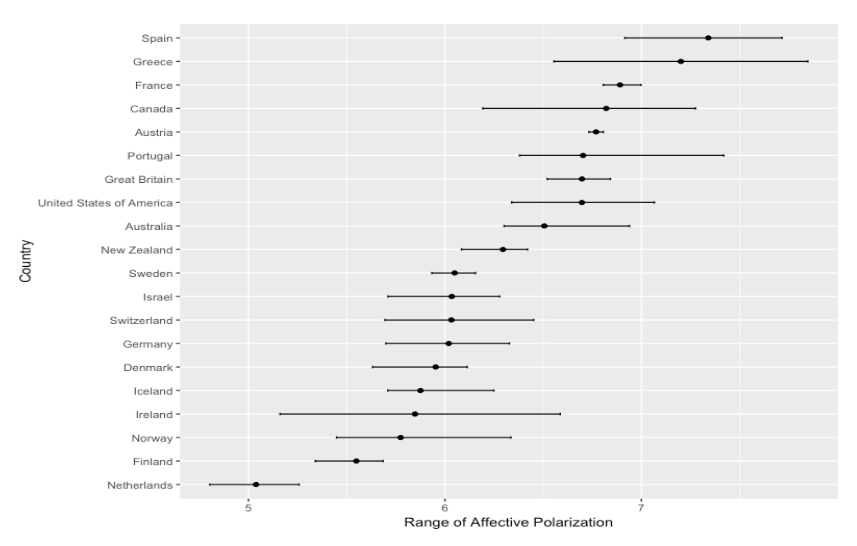
\includegraphics[scale=.7]{figure1.png}
\caption{\label{fig:af-pol-comp} Levels of affective polarization across countries. Source: \cite{Gidron2018}}
\end{figure}

Affective polarization has been well-documented since 2012 --specially regarding its causes--, at least in the US \citep{Hetherington2015,Rogowski2016, Webster2017,Lelkes2018,Iyengar2019, Klein2020}. However, scholars in Europe --and also in Spain-- have only started to focus on this issue recently, although as \cite{Miller2019} points out, the prominence of the concept makes it the ``political phenomenon of the moment". Moreover, little effort has been made investigating the consequences of the phenomenon. Perhaps, the reason behind the lack of studies focused on the consequences of affective polarization is related to poor data (that is the case of Spain), or that's simply because it is a very complex phenomenon that depending on the country can be very correlated with simple ideological polarization and other similar phenomena, making it difficult to disentangle its effects. For example, we already know that 2008 financial crisis had a great impact on the european party systems. In some places like Spain, after more than two decades of stable bipartidism, a multiparty system emerged. This increase in the number of parties confronting in parliament brought altogether a sharp increase of affective polarization which, in the case of Spain, has ended up leading spanish people to polarize even more in two big blocks of parties \citep{Orriols2020}.

The majority of studies addressing this question points out that high levels of affective polarization could be dangerous for democracy. Scholars usually argue that it makes democracy work worse although they do not test in which way. Some exceptions are worth noting though: \cite{Wagner2021} finds that it has an impact on democratic values. Specifically, he finds a negative effect on satisfaction with democracy. Similarly, \cite{Ward2019} find that affective polarization affects perceptions of political choice as well as turnout and participation. Likewise, there is a common intuition in the literature that polarized citizens are less able to collaborate and to work together to solve collective action problems \citep{Garrett2014}. Citizens trust in political institutions and legitimacy of governments are also negatively affected \citep{Orriols2021}. In the same vein, affective polarization can also foster political radicalism \citep{Levendusky2013, Rogowski2016, Webster2017} since the dynamics of polarized politics makes the radicals more prone to speak and, at the same time, it makes polarized --but less radical-- people, more prone to follow the former. There is also a concern regarding satisfaction with democracy, electoral participation, and a long list of attitudes towards western liberal electoral democracy. However, almost none of those pernicious effects of affective polarization have been empirically tested. In this study, I propose a mechanism through which affective polarization may affect different key stages of the democratic process and I try to test one of them.

The general argument is that affective polarization makes people assess political phenomena --and also non-political phenomena-- using their own `political glasses'. Hence, they are less permeable to political information and political cues, or in other words, they are less prone to process political information from a critical standpoint. That is, our own biases are exacerbated because we identify an in-group to which we belong, and an out-group that we see as totally opposed to us. This situation reduces our critical assessment of political --and non-political-- phenomena. Therefore, it has implications in --at least-- three key democratic mechanisms: voting, public policy choice (i.e. preferences) and political support. First, polarized people should be less able to assess government performance and to vote accordingly, so the first implication of affective polarization is related to economic voting but also to accountability itself. Second, they should be less able to place themselves in the ideological scale when affective polarization implies a high party identification which, in turn, makes some citizens be for (or against) policies that are pernicious (or beneficial) for them (i.e. working class people being against universal basic income if the policy is not endorsed by their party). And third, specially during political crisis (of economic, health or other nature) they should be less prone to support the incumbent (unless they voted for it) and, more importantly, the incumbent response to the crisis (measures or policies) that can even be necessary in such a context. This last point has more to do with a lack of civic values like, for instance, the fact that voters against the socialist government of Pedro Sánchez in Spain might have avoid using masks during the pandemic but also organize demonstrations against the government and the measures taken during the pandemic when, in the end, these measures not only were taken under scientific advice (was it correct or not), but to a large extent political consensus also in almost every country in the world.

Hence, the goal of this study is twofold: first, I propose a theoretical mechanism that explains why affective polarization has negative effects on the democratic process. And second, I test empirically if that is the case regarding economic voting (i.e. performance voting). According to the argument, we should see polarized people unable to reward or punish incumbents according to economic performance, that is, we should observe that accountability does not work properly. The remaining of this study proceed as follows: first I present my argument discussing the relevant literature on affective polarization and economic voting. Second, I present my data and experimental design. After that I discuss the main results. Finally, I conclude.
\section{Understanding affective polarization}
\label{affective polarization}

Affective polarization is a fairly new field of research. The concept relates to the fact that citizens feel sympathy towards partisan in-groups and antagonism towards partisan out-group \citep{Wagner2021}. Regardless of its novelty, it has been largely studied in the US. After the work of \cite{Iyengar2012} came out, a lot of different aspects of this phenomenon have been empirically tested in many different countries. However, the vast majority of the literature has focused on the causes, and only a few instances have said something abut its consequences. Also, given the salience of the topic in American politics, scholars have measured affective polarization \footnote{To see a more in depth discussion about the concern about how to measure affective polarization see \cite{Druckman2019a}} mostly in the arguably most straightforward case, the american two-party system \citep{Wagner2021}. However, some authors have recently tried to fill this gap and they have proposed new ways of measuring it in multi-party systems \citep{Reiljan2020}. Moreover, affective polarization is usually addressed at the aggregate level, that is, as the average affective polarization of the political system. Nonetheless, it can also be studied from an individual perspective, since in the end, each individual has a level of affect (or disaffect) for these in-groups and out-group members. \citep{Wagner2021}.

So far, we know that affective polarization is more complex that one might think at first glance. It is neither ideological polarization (although correlation is high in certain contexts), nor party identification (although this is an essential part of it). It is rather something related to social identity. Therefore, it is rooted in political psychology and more precisely in social identity theory \citep{Tajfel1979}. From this standpoint, affective polarization relates to the belonging sentiment to certain social groups. Although it can be the case that belonging to a social group is a matter of ideology, affective polarization is not exactly the same as ideological polarization since people who belong to the same part of the ideological spectrum can have different in- and out-groups. In fact, as some scholarship has shown, in some settings affective polarization can increase while ideological divisions shrink \citep{Levendusky2016, Iyengar2019}. Nonetheless, some other scholarship has shown that ideological polarization impacts affective polarization \citep{Rogowski2016, Webster2017}.

Moreover, affective polarization is not only party identification (i.e. positive in-group affect towards a party and its supporters) because it also relates to the positive or negative out-group affect towards other parties and their supporters. That is, as some have already pointed out \citep{Medeiros2013, Abramowitz2016}, there is `negative partisanship' as well as positive partisanship. Moreover, specially in multi-party systems (in which I am interested here) the in-group and the out-group are not necessarily conformed by one single party each. On the contrary, there can be several combinations regarding the number and the distribution of parties in those groups and, even more importantly, these combinations may be related to country's cleavages in specific contexts and moments like, for instance, Spain and the Catalan secessionist movement during the last 5 years.

\textcolor{red}{Regarding the origins of affective polarization, although this paper is focused on its consequences, a brief comment is worthwhile. There are basically three main sources of affective polarization according to the literature: the high-choice media environment (including cable television and internet), political campaigns, and the polarization of political elites. Some scholars point to the selective consumption of partisan media as the main cause of the increase of affective polarization \citep{Garrett2014, Lelkes2017}. Although mechanisms are not clear and scholars find mixed empirical evidence. Others point towards the effect of political campaigns exacerbating partisan tensions \citep{Sood} and also the positive effect of elections salience on affective polarization \citep{Hernandez2021}. Finally, a growing set of authors put emphasis on the fact that polarized political elites tend to polarize citizens views, fostering affective polarization \citep{Druckman2013, Gidron2018, Rodriguez-Teruel2021}.}



\section{Economic voting (briefly) revisited}

Contrary to what happens with affective polarization, economic voting is not a new issue. According to \cite{Lewis-Beck2018}, we can find studies dating as far back as 1878. But the pioneer papers on the topic are very well known since the 1930s \citep{Tibbitts2015, Gosnell1940, Wilkinson1950}. However, the first scientific proposition of the relationship between the economy and electoral results was placed in a chapter of the seminal \textit{The American Voter} by Campbell et al. (\citeyear[Chapter 14]{Campbell1960}), where they even suggest that economic prosperity is associated to the incumbent presidential party. Since then, a huge literature has been produced on economic voting. Moreover, the classical theory has received considerable empirical support \citep{Kinder1979, Lewis-Beck1988, Lewis-Beck2000, LewisBeck2007, Lewis-Beck2011}. The basic claim of this theory is based on rational choice theory and says that voters, trying to maximize their utility, would vote accounting for the government economic performance. This is usually understood as one of the main accountability mechanisms in western liberal democracies. When economy goes bad, voters punish incumbents, whereas when they do well, voters reward them.

A similar way of putting the core argument of this theory is looking at one of the main `stylized facts' about economic voting, which is the following: retrospective voting is usually more important than prospective voting \citep{Lewis-Beck2000}. This is sometimes called the `responsability hypothesis': voters hold the government responsible (i.e. accountable) for economic events. Hence, according to this theory, we should observe that voters properly assess the performance of the incumbent and vote accordingly. 

However, some scholarship has already pointed out that economic voting is influenced by the context \citep{Dorussen2002, Anderson2007, Singer2015}. \cite{Dorussen2002} argue that the most explosive growth of the economic-voting literature was, interestingly, related to the emergence of controversies about the nature of the economic-voting calculus. Although previous literature had proved that economic performance had such an important salience among the electorate to influence election outcomes, it was not clear which economic policies matter most to voters. Also, it was far from clear if this salience vary accross groups of voters, electoral contexts and political systems \citep{Dorussen2002}.

According to this literature, we shouldn't look at the relation between vote and economy isolated, but accounting for contextual factors. As \cite[p. 1]{Singer2015} point out, ``there is still a debate about whether voters focus on past or future performance and whether they view the economy in primarily sociotropic or egotropic terms". They find that prospective voting predominates early in the election cycle and retrospective voting gains traction as people observe incumbent's performance. Moreover, they also find that sociotropic views predominates over the egotropic ones except for the least developed countries. In the same vein, in a provocative paper, \cite[p. 1]{Anderson2007} argues that economic voting does not work as `envisioned by advocates of democratic accountability'. He  calls for a reconsideration of the normative underpinnings of economic voting paradigm in light of recent evidence. His argument is that although the findings supporting empirically the theory enumerated above exist, they are contingent for both institutional and psychological reasons. I try to disentangle both in this study and focus on the latter.

Nonehteless, the core `empirical asumption of the theory still holds. It is more likely to find people voting retrospectively than prospectively. Only when people observe incumbent's performance they start thinking in voting in prospective terms. As I would argue in the next section, it is reasonable to expect that retrospective voting (and economic voting in general) is less important as people is more polarized. The more polarized they are, the less able they are to assess economic performance. I expect to see voters to use some other strategies and shortcuts in order to maximize their utility. Although this is not to say that they will achieve their goal, contrary to what happen with center oriented and instrumental (i.e. `rational') voters, polarized individuals should avoid to a larger extent the use of information to make their final decision and cast their votes.

\section{Argument}

Once I have presented the most relevant literature to understand affective polarization and economic voting, the linking nexus must be analyzed. I argue that affective polarization has a direct effect on political attitudes, more specifically on the way citizens assess political (and economic) performance, because it activates a process of motivated reasoning (see Figure \ref{fig:model}). 

\begin{figure}[H]
\centering
\begin{tikzpicture}
		\node  (0) at (-5, 0) {Affective Polarization};
		\node  (1) at (0, 0) {Motivated Reasoning};
		\node  (2) at (5.5, 0) {Poor economic voting assessment};

		\draw [style=basic arrow] (0) to (1);
		\draw [style=basic arrow] (1) to (2);

\end{tikzpicture}
\caption{\label{fig:model} Effect of affective polarization on Economic Voting}
\end{figure}

Motivated reasoning is usually studied in cognitive science and social psychology and refers to the fact that some people use emotionally biased reasoning to produce justifications (or make decisions) that are most desired rather than those that accurately reflect the evidence \citep{Kunda1990}. In my setting, this is reflected by the fact that `affectively' polarized people are so according to their emotions, that is, to the level of animosity against both the in-group and the out-group. They would use motivated reasoning to avoid being at odds with their in-group. They would prefer to be `loyal' to their in-group than to punish them if economic situation goes bad. Or the other way around, they would avoid rewarding their out-group when economic performance was good. In other words, those more polarized are expected to use motivated reasoning to a larger extent and hence, would be less able to process (i.e. evaluate) and integrate political (or economic) information. They will be less willing to hold their party accountable for policy performance. That is, this motivated reasoning would lead them to vote in a less rational way, or in other words, economic voting will work worse. It is also reasonable to expect partisans to undermine rather than promote responsible government. 

Nonetheless, there is a major issue with the causal chain proposed. As I discuss in the next subsection, we already have some evidence of motivated reasoning being the cause of political polarization. This is not exactly a problem of reverse causality since, in the end, the combination of both --affective polarization and motivated reasoning-- is what would influence economic voting. However, it is important to dig deeper into the concept of motivated reasoning in order to clarify the causal mechanism and the causal chain proposed as much as possible.


\subsection{Motivated reasoning}

As suggested by many scholars \citep{Taber2006, Boyer}, reasoning seems to play a crucial role in the formation of political attitudes. Citizens are not only motivated in the sense of holding \textit{accurate} beliefs, but also ``\textit{directional} motivations, or motivations to reach a certain predetermined belief" \citep[p.2]{Boyer}. Such directional motivations are, according to \cite[p. 440]{Kunda1990}, ``any wish, desire or preference that concerns the outcome of a given reasoning task". In order to better understand the underpinnings of the process by which polarized people activate a motivated reasoning process, it is interesting to discuss the different effects that positive and negative partisanship may have.

As noted before, affective polarization is not only a matter of hate or dislike, it also may increase due to a reinforcement of individual's positions and views being closer to his/her party, that is, an increase of positive partisanship. Some authors have already studied the effect of motivated reasoning focusing on the level of trust and how people process Fake News \citep{Thaler2021}. He finds that motivated reasoning from political messages on topics like immigration, income mobility, crime, racial discrimination, gender, climate change, gun laws and performance of other subjects, leads to people's beliefs to become more polarized \citep{Thaler2021}. According to him, the causal chain would be slightly different since polarization would be a byproduct of such psychological process or bias. However, I am not totally sure this is the case. I think that when a certain level of affective polarization (probably different in each country and context) is reached, the context fosters or reinforces this psychological bias, hence, motivated reasoning can bring political polarization at first, but after a certain threshold, a feedback loop is produced. Thus, in countries where affective polarization is very high, I expect this context to be the cause that exacerbate the psychological bias that ultimately would lead people to assess economic events in a \textit{non-rational} way. We also have evidence that motivated reasoning could be the cause of polarization when focusing on Identity Politics. \cite{Boyer} find that group status is a powerful moderator of political motivations. High-status groups members --for instance, men compared to women-- are more strongly motivated, which leads them to political polarization between left-wing and right-wing more easily \citep{Boyer}.

However, if we look at the characterization of motivated reasoning proposed by \cite{Thaler2021}, we would find that the causal chain proposed in Figure \ref{fig:model} is valid. He argues that motivated reasoning ``posits that people distort their inference process in the direction of states they find more attractive". Taking this characterization, we see that people active the motivated reasoning process once they find a state considered as ``more attractive". Thus, since affective polarization is a byproduct of the in-group and out-group feelings, or rather, of positive and negative partisanship, this context of affective polarization is required prior to motivate the reasoning. Put it differently, only once people is polarized because they like or dislike a certain party or set of parties (and their supporters), can they motivate their reasoning when assessing, for instance, economic events. The bias is produced once they know which is their in-group and out-group and only then, they direct themselves to a certain state they find more attractive. Nonetheless, this does not restrict the possibility that one of the causes for an individual placing herself in a certain group is related to certain goals or states found ``attractive". In short, what I argue is that a context of affective polarization can reinforce the psychological process by which biases make people more unable to process new political information.

\subsection{Elasticity}

I introduce now the concept of elasticity to try to shed light on the economic voting part of the argument. I use the term elasticity to refer to the extent to which people is permeable to political information. Polarized people is, in general, less permeable to political information, specially when this information is at odds with their prior beliefs. This is to say --in Bayesian terms-- that they (almost) do not update their priors. Moreover, I argue that when political polarization is not only about policy choice, but also related to affects, (lacking) permeability turns into (lacking) elasticity. These two concepts, may look the same at first glance but I would try to elaborate a bit more on the distinction in what follows.

Someone less permeable to political information may reject information coming from a political opponent, for instance a party leader, a congressman of the (or one of the) opposing party (parties), etc. However, someone inelastic with respect to political information is someone that not only does not trust political opponents but other sources of information either. These inelastic (i.e. \textit{affectively} polarized) people, would not accept information at odds with their beliefs even when it comes from a \textit{a priori} neutral source of information. The bias in this kind of people is much stronger and applies immediately. As soon as the information received goes against their in-group or the party they vote for, they do not trust it or do not believe it. In the same vein, information against their opponents is taken as an absolute truth, regardless of their party leaders making this information. In short, elasticity is a stronger effect when it comes to process political information. That is because one can be slightly permeable but not necessarily unable to assess the data or information, whereas someone inelastic is characterized as someone unable to assess rationally even external (i.e. non partisan) sources of information.

\subsubsection{Elasticity and positive and negative partisanship}

Moreover, elasticity may be different regarding in-group and out-group feelings. That is related to the distinction between positive and negative partisanship. As stated above, affective polarization is not only a matter of one of the two, but can be (and so I argue) a combination of both. This can yield different results and profiles. There is people that is polarized because they like their in-group very much (i.e. positive partisanship), people that is polarized because they dislike their opponents a lot, or even hate them (i.e. negative partisanship) or a combination of both. The latter would be the most strongly polarized, whereas polarization levels in the other two profiles may vary. Hence, it is expected to find what I call \textit{supporters}, people with average to high levels of elasticity; what I call \textit{partisans} with average levels of (lack of) elasticity and \textit{fans}, with very low levels of elasticity. In short, elasticity is a function of positive and negative partisanship. One of the goals of the present study is to disentangle these effects in order to better understand affective polarization when it is decomposed in its two constituent components.


\section{Hypotheses}

The main hypothesis I test in this study is the following:

H1: \textit{Those more `affectively' polarized are less prone to reward (punish) the incumbent according to economic performance.}

Some additional hypotheses subject to be tested are related to disentangling the two main components of affective polarization, namely, positive and negative partisanship. Since it is possible that economic voting works even better or more ``strongly" among those who didn't vote for the incumbent, it is important to highlight that the goal of the paper is to compare the level of affective polarization among all the people that didn't vote for the incumbent. Conversely, we need to compare the level of polarization of those who voted for the incumbent and, for both groups, check the level of economic voting. That is, the level of economic voting is not an absolute measure but a relative one. It is relative to the level of affective polarization of those in the in-group and out-group respectively.

Thus, I can test if among the most polarized economic performance is less important. However, the effects don't have to be necessarily of the same size. It is reasonable, for instance, to find that among the opposition voters economic voting is more important on average than among supporters for the incumbent. This is because even people who is not very polarized is less willing to support a government that they didn't vote. The important measure here is the level of congruence between real economic data and incumbent performance and individuals economic assessment. 

However, the general argument I have posited here, can be tested --I argue-- looking at many different outcomes. I expect affective polarization to have a similar effect on --at least-- three key stages of the democratic process: voting, preference formation and political support (see Figure \ref{fig:general-model}). 

Hence, some other tentative hypotheses that are plausible to be tested in future research [perhaps as part of a PhD proposal] are the following:

\textit{H2: Those more `affectively' polarized are less likely to support a certain policy when it is endorsed by a party ideologically close but that belongs to the out-group.}

This hypothesis comes from the intuition that specially in multiparty systems in-groups and out-groups can be fairly heterogeneous. Thus, there are situations in which people who place themselves in a certain side of the ideological spectrum, are against measures proposed by parties that belong to the out-group only for this reason. That is, even when a policy like, for instance, the universal basic income, can be potentially beneficial for low income people, this people may be against this policy if it is proposed by an incumbent supported by a party different from which they vote for. This may be specially the case in a context of high affective polarization.

\textit{H3: In times of crisis, those more `affectively' polarized are in general, less supportive of the incumbent measures regardless of the level of `partisanship of the policy'.}

This hypothesis refers to the fact that in bad times, some measures are taken not necessarily from a partisan perspective, but as necessary temporal measures. Think, for instance in the COVID-19 lockdowns. Although one can argue that incumbents can decide whether to impose such a measure in a partisan way, the measure is equally imposed to everyone, supporters and opponents. Hence, very polarized people is expected to be less willing to accept this kind of measures, although in the case of a health crisis like the one we are living right now, those measures might be necessary. I acknowledge that this hypothesis may be controversial if it is wrongly understood. I am not claiming that people should accept incumbents measures \textit{tout-court}. I am rather arguing that some measures not taken as partisan, are understood as partisan by those more polarized. This may have implications in terms of political attitudes.

\begin{figure}[H]
\centering
\begin{tikzpicture}
		\node    (0) at (-5, 0) {Affective Polarization};
		\node    (1) at (0, 0) {Motivated Reasoning};
		\node    (2) at (5.5, 2) {Economic voting};
		\node    (3) at (5.5, 0) {Public policy choice};
		\node    (4) at (5.5, -2) {Political support};

		\draw [style=basic arrow] (0) to (1);
		\draw [style=basic arrow] (1) to (2);
		\draw [style=basic arrow] (1) to (3);
		\draw [style=basic arrow] (1) to (4);
		

\end{tikzpicture}
\caption{\label{fig:general-model} General effects of affective polarization on political attitudes}
\end{figure}

Similarly, some important derivations of this mechanism can bring worth analyzing consequences. For instance, if affective polarization levels are sustained over time, it is to expect a certain party realignment. Hence, this could be against the prominent idea of catch-all parties suggested by \cite{Kirchheimer1966}, (also see \cite{Krouwel2003}). In polarized contexts, we should observe that parties are less willing to try to seduce the out-group, consequently, niche parties would be more likely to emerge. Although we already know that the levels of affective polarization are subject to the fragmentation of parliaments \citep{Orriols2020} and hence, it could arise a concern about reverse causality, we don't have much information about the consequences of affective polarization. Therefore, it could be also something to be tested in future research. In the same vein, satisfaction with democracy has been widely thought to be impacted by affective polarization since the public opinion environment generated by the associated distrust can make governments perform worse. Hence, in the long run, people can get dissatisfied with the political system. This could be easily tested looking at measures of specific and diffuse support as proposed by \cite{Easton1975}.



\section{Research design}

A tentative empirical research design is proposed in this section. However, this draft is primarily intended to organize first, my ideas, second, the huge literature written, and third, the paper structure itself. Hence, I am not sure which will be my final research design. Please, take the next comments as suggestions and ways to start working out the results.

Since my main hypothesis refers to individuals, I would use a micro level database to empirically test it. One of the possibilities is to use a very well known international database with electoral data at the individual level: the Comparative Study of Electoral Systems (CSES) database. The five modules of CSES database include elections since 1996 up until today in a lot of different countries. This could be interesting specially if I end up comparing different polarization contexts. In each module a different number of election studies ranging from 31 to 50 are included. Also, they include a number of polities between 28 and 41. All these modules taken together 

This database has been used in the past precisely to get affective polarization measures across countries. The usual way of measuring polarization is the one used by \cite{Gidron2018}. They use survey data from a module asking respondents to rate political parties in the classical 0-10 thermometer scale (that is, how much they like or dislike a certain party). After that, they basically inverse the scale so that 10 denotes the most negative party evaluation and 0 the most positive. However, instead of calculating an average level of affective polarization, I need to compute the individual amount of polarization. That is obtained as a measure of the spread of the affect an individual shows for a certain number of parties, in other words, it is a ``weighted average party affect difference compared to each respondent's weighted average party affect" \citep{Wagner2021}:

$$
\text{Spread}_i = \sqrt{\sum^p_{p=1}\nu_p(\text{like}_{ip}-\overline{\text{like}}_i)^2}
$$

Where $\nu_p$ is the vote share of each party so I can account for party size. Moreover, the mean affect should itself be weighted by party size, calculated as:

$$
\overline{\text{like}}_i = \sum^p_{p=1} (\nu_p * \text{like}_{ip})
$$

This would allow me to compare individuals using their level of affective polarization. Now, In order to check if economic voting `is working' as expected, I need a measure of national economy assessment made by respondents, o more precisely, a relative measure of accuracy assessing the state of the economy. CSES database includes several questions related to economy change or state of economy. Respondents are not asked to give a very precise assessment of the economic situation, they are just asked if they think economy is either better or worse than in the last 12 months. This wouldn't be enough as to compute the level of accuracy assessing the state of the economy. In order to achieve that, perhaps a comparison between individual's answer and macroeconomic indicators of the country would be informative as to what extent the assessment was accurate. This relative measure could bring some insight about the level of economic voting from one election to another for each individual.

Moreover, the CSES modules include a considerably big set of political variables useful to be introduced as other regressors or even controls. I have available, for instance, variables such as party choice made for the respondent, if they voted for the incumbent or not in the last election, if he/she is a switcher between elections, etc. Furthermore, this dataset has also available a very big amount of sociodemographic controls that would be essential for the study.

However, there is an important downside of this approach: CSES data is very good to make cross-country comparisons, but it is not panel data. Nonetheless, there is a different approach that could also be implemented as my research design. Using the E-DEM dataset, a new micro-level online panel survey of the Spanish voting age population with more than 8.109 interviews collected \citep{Torcal2020}, I could track individuals' opinions and their assessment of the economy during a crucial period in Spanish recent politics. This dataset contains four waves spanning a period between October 2018 and May 2019. During that period of time, most of the key political events affecting Spanish politics after 15M happened: for instance, local, regional, national and European elections took place within this period, but also the conviction of Catalan secessionist leaders. And, more importantly, it also covers the six-month period of surge of Spain's new radical right party, Vox \citep{Torcal2020}. This last event is expected to be very related to the uprisal of affective polarization levels in Spain (either as a cause or a consequence).

This dataset also contains both variables capturing individuals assessment of the economy, with the advantage of being panel data, and a lot of sociodemographic and attitudinal variables useful for controls. However, it also has a downside. Although there are questions about leaders' assessment and party identification, there is no thermometer scale included. I could use though some questions about ``feelings towards people from certain regions, voters of certain parties, and party leaders" as a different measure of affective polarization. In fact, I think that specially for the case of ``feelings towards voters of different parties", this would be an even more accurate measure of affective polarization as described in section \ref{affective polarization}. The scale is slightly different, it ranges from 0 to 100 with jumps of 15 points. Nonetheless, this measure could still fit \cite{Wagner2021}'s formula.

Hence, there are two possibilities, either using a cross-country database in order to add a comparative perspective in the study using the classical measure of affective polarization, or stick to the spanish case (which I find sufficiently interesting regarding affective polarization, see \cite{Orriols2020}) and take advantage of panel data in order to track individual's assessment of the economy, voting behavior and level of affective polarization. In either way, the model to be estimated is not decided yet.

In order not to lose the contents describing the CSES database, I decided to keep both possibilities in the present section. However, for the next sections, it is important to note that the first empirical exercise is done using \citep*{Torcal2020} data for the Spanish case.

I sumarize some descriptive statistics as well as my main results. Regarding the latter, the design consist of a simple logit model which outcome variable is a dummy variable capturing whether the respondent would vote for the incumbent or not. Hence, I estimate the probability of voting for the incument subject to the assessment of the economy, a classic way of test economic voting hypotheses. 

It is important to note that this variable is constructed in a rather convoluted way because of data constraints. Ideally, I would use either actual vote recall or vote intention in a certain election. However, since the timespan of the survey only covers April 28th national elections, I have combined two different variables to construct my dependent variable. For the third wave of the survey, there is a question about vote intention in April's elections, hence, I code a one if the respondent answers that he or she is thinking to vote for the PP (the incumbent at that time) and a zero otherwise. However, to be able to use a considerable part of the dataset that otherwise would have been lost, I use the declared probability of ever voting for a certain party to code those respondents in wave four. Wave four happened after the 28th April elections. Sadly, there is not a question asking for vote intention in the November the 10th elections. Thus, I code a one if the respondent probability of voting for either PSOE or UP is grater or equal than 5 (the variable ranges from 0 to 10). I think that this is important specially because some of the key questions about feelings towards VOX voters are only present in the fourth wave since the party was a newcommer in April election.

Therefore, the model to be estimated is as follows:

\begin{equation}
	\label{model}
	y_i = \beta_1 x_{1i} + \beta_2 x_{2i} + \beta_3 Z_i  + \eta_i  + \epsilon_i
\end{equation}

where $y_i$ is the already described outcome variable, $\beta_1$ is the expected effect of econmic voting\footnote{Measured as the individual's assessment of the spanish economy. The question wording is: \textit{And, how has the economic situation in Spain changed in the last 12 months?} Answers range from 1 "A lot worse" to 5 "A lot better"} alone, $\beta_2$ is the effect of affective polarization index on the probability of voting for the incumbent and, the outcome of interest, $\beta_3$ is the interaction between both $x_1$ and $x_2$. Thus, $\beta_3$ capture the effect of economic voting according to the level of affective polarization of the individual. Finally, $\eta_i$ is a vector of sociodemographic and attitudinal control variables, and $\epsilon$ is the error term.

\section{Descriptive Statistics}
\label{section:descriptive}
To start with the exploration of the Spanish data, in Figure \ref*{fig:feelings} we can see the distance in feelings towards voters of each party for those whose level of affective polarization is above and below the average. This is an important measure because reveals the extent to which positive and negative partisanship is present in the Spanish system. The horizontal axis plots the level of warmess that an individual has regarding voters of every one of the four biggest parties. It ranges from 0 being feeling very cold to 100 being feeling very close or warm. In the vertical axis I separate the results for each party to explore the plausible heterogeneity. The parties are ordered according to their posistion in the ideological scale (left to right is top to bottom) in order to ease the interpretation of the results. The results are somewhat mixed although they can give us some insight to explain later the main empirical findings. 

First of all, there is a common pattern among parties and their supporters. As we could expect, those more polarized than the average tend to have stronger sympathy for their party's voters. This is the case for all the parties except for VOX for which the distance between more and less polarized is not statistically different from zero at the 90\% level. It looks like --at least for the Spanish case-- positive partisanship is working powerfully.

\begin{figure}[H]
	\centering
	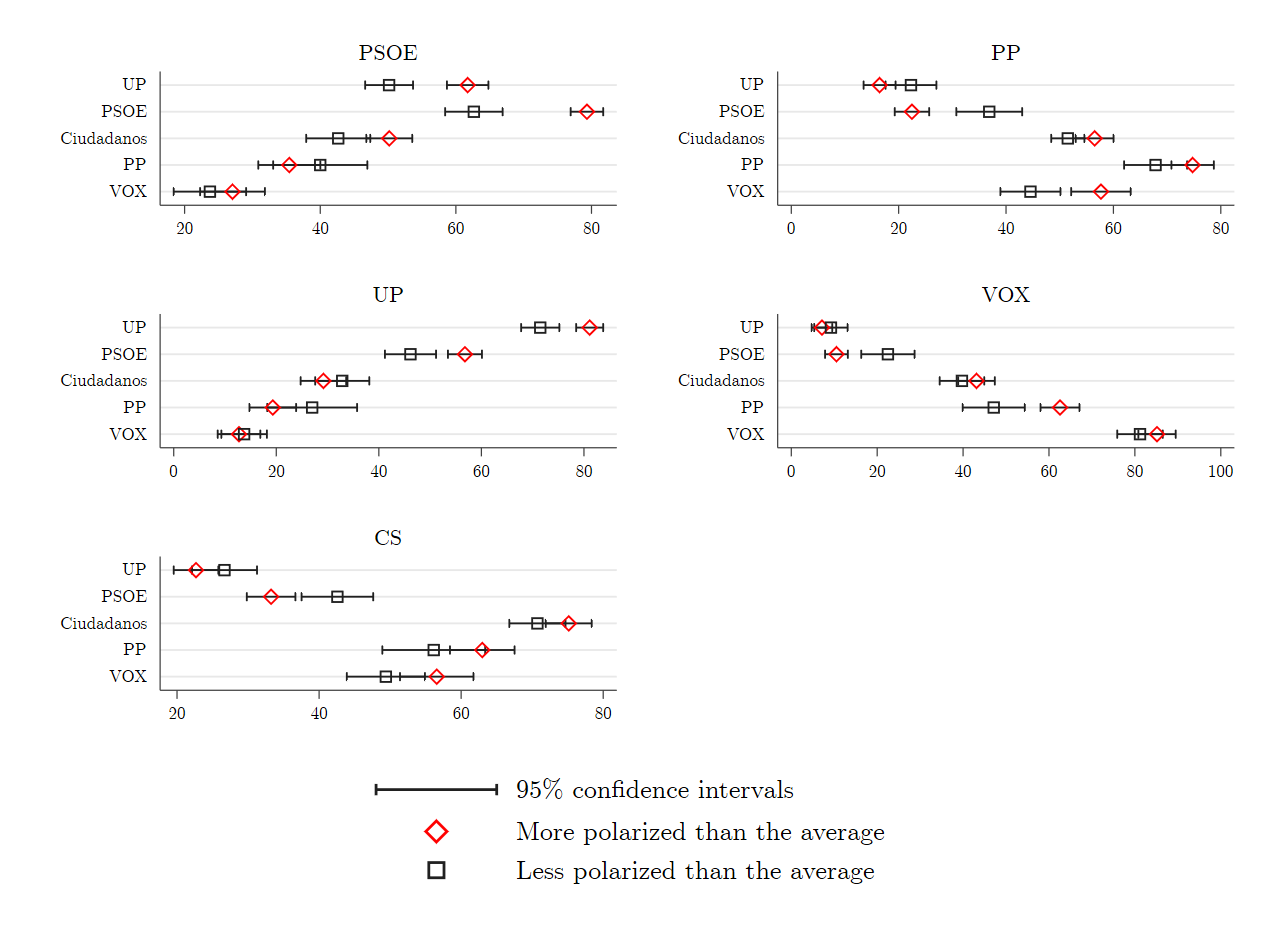
\includegraphics[scale=0.35]{Figures/combinedfeelingsAP.png}
	\caption{\label{fig:feelings} Feelings towards party voters and affective polarization}
\end{figure}


Now, although most of the distances measured are not significantly different from zero, we see some clear patterns in the data. For example, looking at the two main traditional parties (PP and PSOE) we see that those more polarized tend to have colder feelings towards voters of the other party. This offers a clear --and if anything conservative-- measure of the level of polarization between the two main parties which, in turn, are the most moderate on average. It is important to note that the difference is grater in the case of PP voters. This suggest that maybe ideology might have an effect on the magnitude of the distance between more and less polarized. 

The reason of ploting parties ordered by ideology in the vertical axis is to better see that except for Ciudadanos who is put at the end of the panel on purpose, we see a mirror image on the pattern. In line with \citep*{Orriols2020}, there is a clear pattern regarding the outgrup formation that basically has to do with two ideological blocks. If we look at Figure \ref*{fig:feelings} by rows, we see that left parties' voters display feelings that are a mirror image of those of the rightwing voters. Moreover, the spread of those feelings, in line with \citep*{Wagner2021} is grater as the parties move appart ideologically, that is, feelings towards both the in-group and the  out-group are more extreme for UP and VOX voters than they are for PSOE and PP respectively. Finally, Ciudadanos' voters are, interestingly, those who display the most statistically significant results. However, it is very relevant to see that contrary to what one might expect, the most ``centrist'' voters tend to be closer to right wing parties and further away from leftwing parties the more polarized they are. This, nonetheless, could be explained by the the timing of the data. Since the period covered by this survey includes the most vibrant moments of the secesionist movment in Catalonia, it is reasonable to see Cs voters more polarized on average than the rest of voters since, as we know, the territorial dimension is one of the most polarized in Spain.

\section{Results}

Now we turn to the main results of the paper. In this section I sumarize and discuss the empirical evidence for or against the main hypothesis which is: \textit{Those more `affectively' polarized are less prone to reward (punish) the incumbent according to economic performance.}

\begin{table}[H]
	\label{coefplot}
\centering
\caption{\label{tab:regression} Effects of affective polarization on economic voting}
{
\def\sym#1{\ifmmode^{#1}\else\(^{#1}\)\fi}
\begin{tabular}{l*{3}{c}}
\toprule
                & Baseline         &+ Sociodemografic controls         &+ Attitudinal controls         \\
\midrule
Intention to vote for the incumbent&                  &                  &                  \\
Economic voting &    0.363\sym{*}  &    0.350\sym{*}  &    0.347\sym{*}  \\
                &   (2.37)         &   (2.26)         &   (2.19)         \\
AP index        &    0.455\sym{***}&    0.492\sym{***}&    0.483\sym{***}\\
                &  (14.37)         &  (15.08)         &  (14.52)         \\
Economic voting $\times$ AP index&  -0.0101         &  -0.0227         &  -0.0370         \\
                &  (-0.30)         &  (-0.66)         &  (-1.05)         \\
Sociodemografic controls&                  &      Yes         &      Yes         \\

Attitudinal controls&                  &                  &      Yes         \\

Constant        &   -2.400\sym{***}&   -2.665\sym{***}&   -2.835\sym{***}\\
                & (-17.34)         &  (-8.34)         &  (-8.39)         \\
\midrule
Pseudo \(R^{2}\)&    0.080         &    0.091         &    0.102         \\
Observations    &     3622         &     3622         &     3607         \\
\bottomrule
\multicolumn{4}{l}{\footnotesize \textit{t} statistics in parentheses}\\
\multicolumn{4}{l}{\footnotesize \sym{*} \(p<0.05\), \sym{**} \(p<0.01\), \sym{***} \(p<0.001\)}\\
\end{tabular}
}


\end{table}

As we can see in Table \ref*{tab:regression} I present the results of estimating equation \ref*{model} first without controls and then adding progresively sociodemographic and attitudinal controls. In the three models, the effect of economic voting is positive as expected, meaning that those that evaluate the econonmy as better than in the last twelve months, are more likely to vote for the incumbent. Furthermore, the affective polarization index measured (following \citep*{Wagner2021}) as the weighted average party affect difference compared to each respondent's weighted average party affect has a positive effect on the likelihood of voting for the incumbent, suggesting that those more polarized are, probably, also more engaged in politics.

\begin{figure}[H]
	\centering
	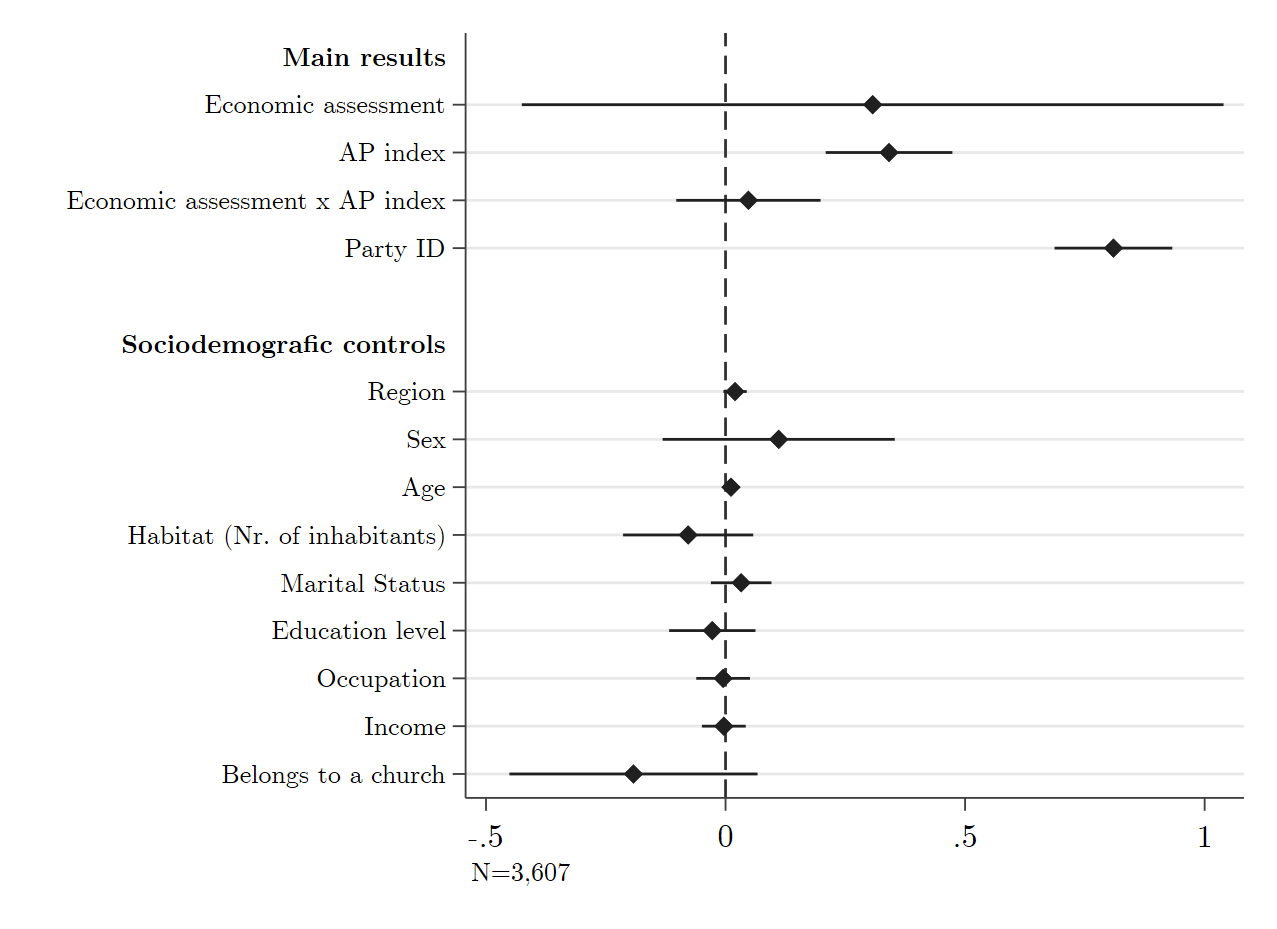
\includegraphics[scale=0.35]{Figures/model_3_coefplot.png}
	\caption{\label{fig:coefplot} Economic voting and affective polarization (Full specification)}
	\end{figure}

However, the main quantity of interest, namely, the interaction between these two terms, is not significantly different from zero at the 95\% level. It is, nonetheless, interesrting to note that the sign of the interaction is, as hypohtetisized, negative. This would mean that as people is more polarized, they are less able to use economic voting in the proper (or rational) way. This flip in the signs of $\beta_1$ and $\beta_2$ would suggest that, according to my theoretical expectations, those more polarized are less able to vote critically.

Since the main question of interest is not statistically significant, I only present here the raw coefficients of the logistic regression estimates. However, to have a notion of the magnitude of the effects, I present odds ratios in Table \ref*{tab:oddsRatio}, in the appendix.

Finally, to better see the results, I present now a coefficients plot. As we can more clearly see in Figure \ref*{fig:coefplot}, the intereaction term is indistiguishable from zero.

\subsection*{Marginal Effects}

Although the main hypothesis does not received empirical support, I also explore the marginal effects of economic voting separating those more and less polarized than the average. In Figure \ref{fig:margins} we can see that, interestingly, the likelihood of voting for the incumbent is much different for these two groups. While less polarized people tend to display ``expected'' marginal effects, meaning that the plotted line crosses the 0.5 probability around values in the middel, those more polarized apparently are much more willing to vote for the incumbent. Even for those whose assessment of the economy is negative, the probability of voting for the incumbent is grater than 0.5. This suggests, in line with the already discussed results in section \ref*{section:descriptive}, that positive partisanship is playing the decesive role here. 


\begin{figure}[H]
\centering
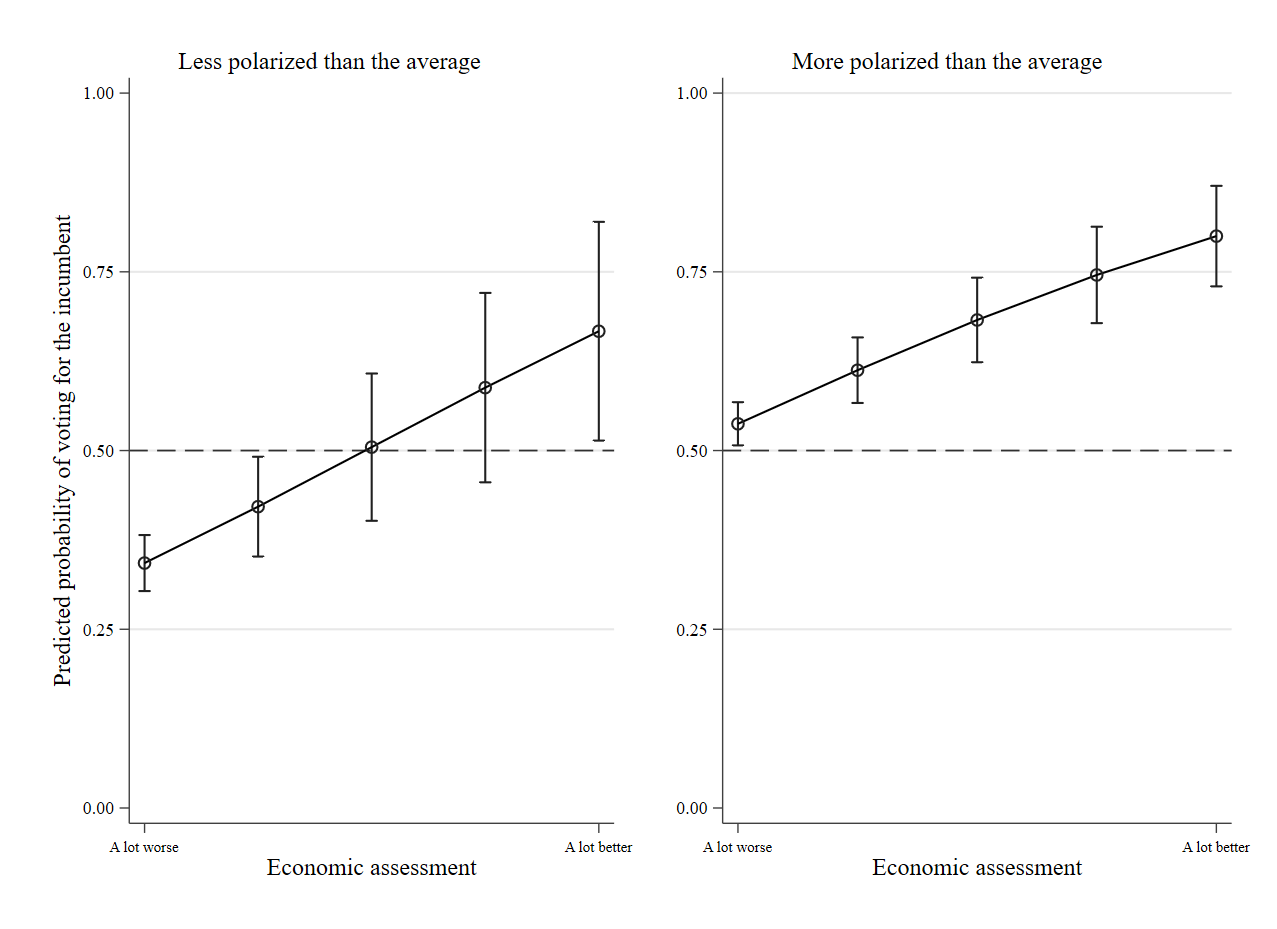
\includegraphics[scale=0.35]{Figures/marginsplot.png}
\caption{\label{fig:margins} Marginal effects of economic voting and level of polarization}
\end{figure}


\section{Broader discussion and possible implications}

All in all, I think that this paper can contribute to our knowledge about affective polarization as such, and more specifically I can push the  frontier of knowledge forward by analyzing its consequences. This piece of work can have even broader implications since it speaks to the general question of accountability itself. I tend to agree with Robert Fishman that economic voting is not always good. Or, in other words, the fact that polarized people would be less prone to vote ``rationally" according to the economic voting logic is not necessarily something good for our democracies. Nevertheless, looking at the amount of literature proving empirically the importance of economy as a tool for the voter to punish or reward politicians in the government, I still think that economic voting is somewhat related to accountability. Accountability is by no means the only desirable feature of a democratic system, but \textit{ceteris paribus}, it is better to have accountability than not to have it. Moreover, the lack of accountability I predict in this study is related to people's lack of elasticity when it comes to critically analyze the economic situation. If people is not able to punish or reward incumbents due to biases and polarization, in general terms, I would say it is a bad outcome for our democracies.

I believe that analyzing the consequences of affective polarization and its effects on political attitudes can open an inspiring intellectual debate about the perils of the phenomenon and the available tools we have to avoid the erosion of our democracies. 

\newpage
\bibliographystyle{apalike}
\bibliography{RIP.bib}


\newpage

\section*{Appendix}

\begin{table}[H]
	
\centering
\caption{\label{tab:oddsRatio} Odds Ratios of voting for the incumbent}
{
\def\sym#1{\ifmmode^{#1}\else\(^{#1}\)\fi}
\begin{tabular}{l*{3}{c}}
\toprule
                & Baseline         &+ Sociodemografic controls         &+ Attitudinal controls         \\
\midrule
Intention to vote for the incumbent&                  &                  &                  \\
Economic voting &    1.438\sym{*}  &    1.420\sym{*}  &    1.415\sym{*}  \\
                &   (2.37)         &   (2.26)         &   (2.19)         \\
AP index        &    1.576\sym{***}&    1.635\sym{***}&    1.622\sym{***}\\
                &  (14.37)         &  (15.08)         &  (14.52)         \\
Economic voting $\times$ AP index&    0.990         &    0.978         &    0.964         \\
                &  (-0.30)         &  (-0.66)         &  (-1.05)         \\
Sociodemografic controls&                  &      Yes         &      Yes         \\
Attitudinal controls&                  &                  &      Yes         \\
Constant        &   0.0907\sym{***}&   0.0696\sym{***}&   0.0587\sym{***}\\
                & (-17.34)         &  (-8.34)         &  (-8.39)         \\
\midrule
Pseudo \(R^{2}\)&    0.080         &    0.091         &    0.102         \\
Observations    &     3622         &     3622         &     3607         \\
\bottomrule
\multicolumn{4}{l}{\footnotesize Exponentiated coefficients; \textit{t} statistics in parentheses}\\
\multicolumn{4}{l}{\footnotesize \sym{*} \(p<0.05\), \sym{**} \(p<0.01\), \sym{***} \(p<0.001\)}\\
\end{tabular}
}

\end{table}


\end{document}